L'interfaccia grafica è realizzata tramite il framework \glock{Angular}, per questo motivo, il design architetturale utilizzato è il \textit{Model View ViewModel} (\textit{MVVM}) che è intrinseco nel framework stesso. \\
La comunicazione con il server avviene tramite \glock{WebSocket} ed è dunque asincrona. 
Inoltre, per garantire l'estensibilità del codice, il servizio \textit{WebSocketService} implementa l'interfaccia \textit{ServerService} che mette a disposizione i metodi per interfacciarsi con il server. In questo modo un cambio di tecnologia, ad esempio passando a richieste \glock{HTTP}, non comporterebbe uno stravolgimento dell'architettura. \\
Per lo stesso motivo sono previste delle interfacce per rappresentare i vari tipi di messaggi che vengono ricevuti dal server, successivamente implementate per specificarne le caratteristiche. \\
Ogni componente che fa parte del \textit{ViewModel} rappresenta una funzionalità principale che l'interfaccia mette a disposizione all'utente.\\
 L'aggiornamento dei dati tra gli \glock{Angular Components} ed il \glock{WebSocket} avviene tramite l'uso dei \glock{Subject} (uno per tipo) al'interno di quest'ultimo; indirizzando tali dati  ai componenti che prevedono appositi campi dati per ricevere le informazioni.\\
\newline
Di seguito illustriamo due diagrammi delle classi: il primo per descrivere il legame tra \textit{Model} e \textit{Viewmodel}, con la struttura dei vari \glock{Angular Components}, mentre la parte di \textit{View}; che comprende i templates degli \glock{Angular Components}, non viene qui rappresentata perché la struttura del codice è \glock{HTML}.
Il secondo, invece, rappresenta i messaggi che vengono inviati e ricevuti dal server.
\newpage

%\begin{landscape}
%	\begin{figure}[h!]
%		\includegraphics[width=25.5cm]{img/ui_modelview.png}
%		\caption{Architettura dell'interfaccia - Model-View Model}
%	\end{figure}
%\end{landscape}
%\newpage

%\begin{landscape}
%	\begin{figure}[h!]
%		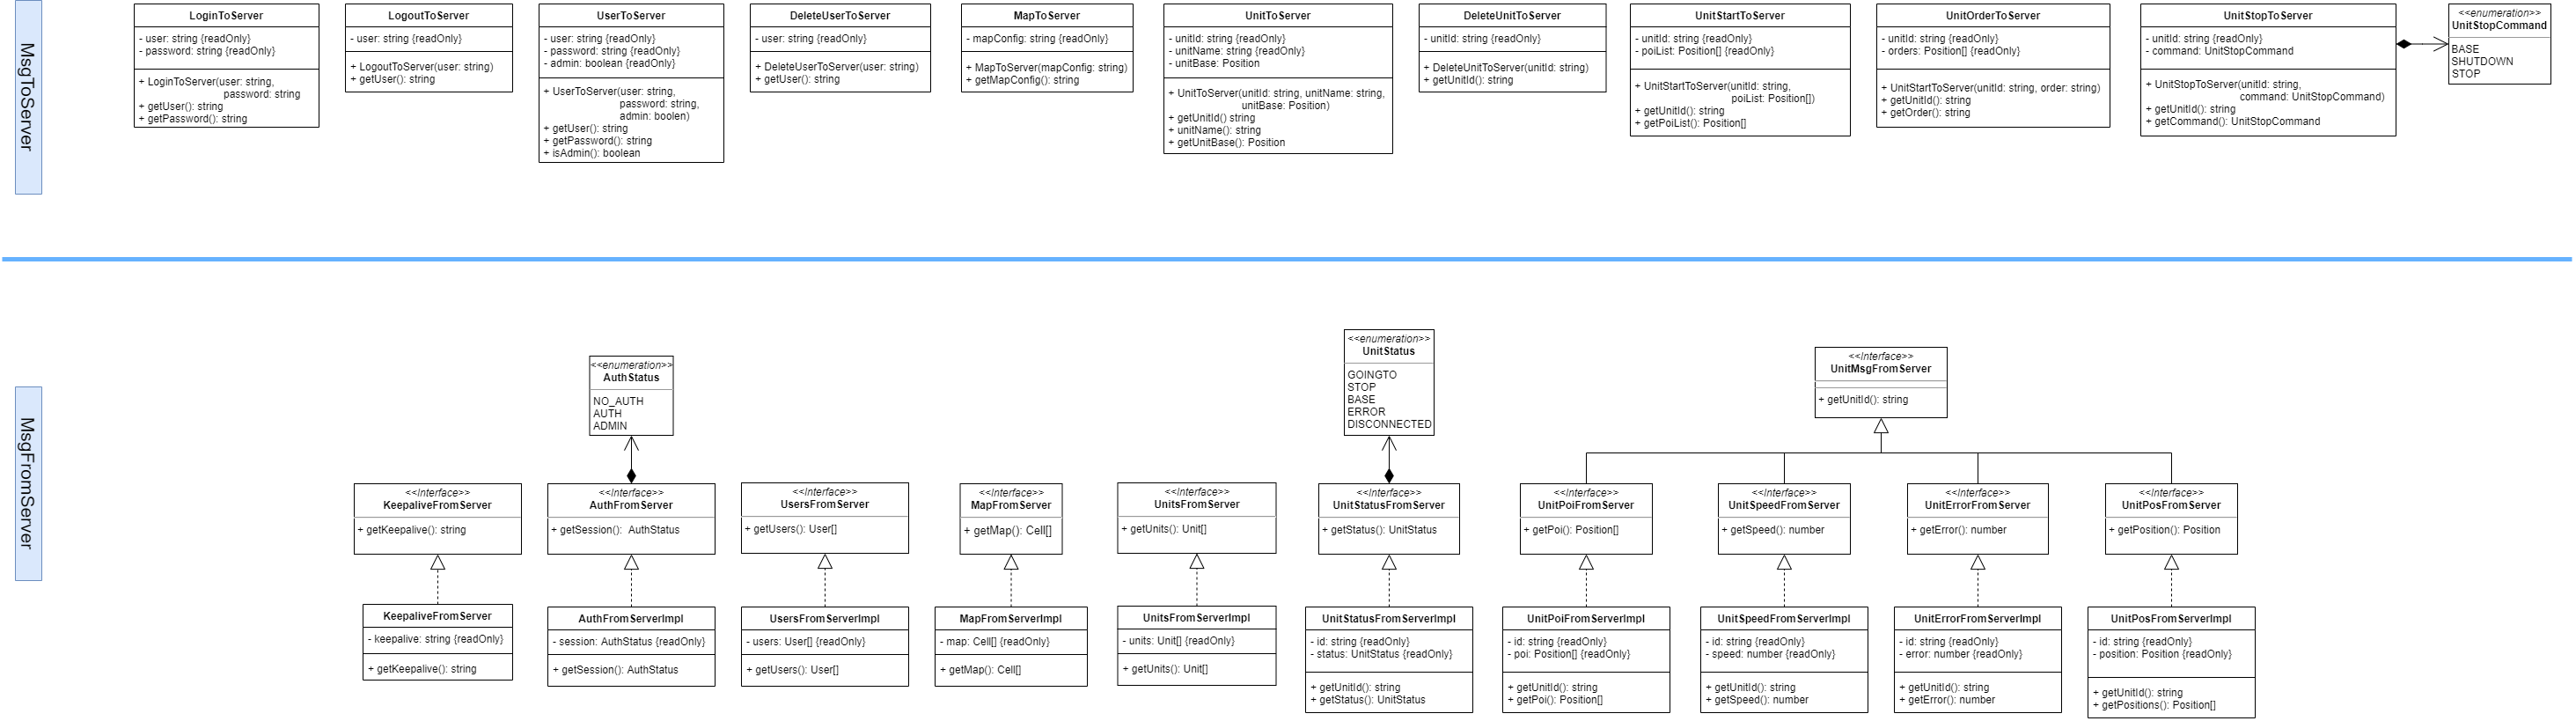
\includegraphics[width=25.5cm]{img/ui_messaggi.png}
%		\caption{Architettura dell'interfaccia - Messaggi}
%	\end{figure}
%\end{landscape}